% -*- Coding: UTF-8 -*-
% Project: hitszthesis_undergraduate
%
% Author: Shawn
%

% 导言区设置
% --- Class Info. ---
\documentclass{style/thesis_ug}

% --- Special package ---


% --- Doc Info. ---
% 由于封面比较难排版,可由Word或其他方法添加封面
\title{哈工大毕业论文\LaTeX 模板}
\appendanttitle{使用教程} % 标题过长时,将第二行写在这
\author{胡\hspace{\ccwd}韶}
\department{机电工程与自动化学院}
\major{机械设计制造及其自动化}
\stunumber{SZ1603102xx}
\teacher{xx\hspace{\ccwd}教授}
\defensedate{2020年06月09日}

% --- Basic setting ---
%\setlength{\bibsep}{0.2ex}

% --- Personal command ---
\newcommand{\mtb}[1]{%
  \makebox[3em][c]{#1}
}

% --- Options ---
%\infowidth = 6.5cm    % 下划线长度

  


\begin{document}
  % ===== Cover | 封面 =====
  \maketitle


  % ===== Front | 书前部分 =====
  \frontmatter
  % --- Abstract / 摘要 ---
  %% 摘要
%% 本科生毕业论文的摘要,要求用中、英文两种文字给出,中文摘要的字数(以汉字计),一般为300字
%% 左右,以能将规定内容阐述清楚为原则。英文摘要与中文摘要的内容应完全一致,在语法、用词上应
%% 准确无误,摘要页不需写出论文题目。
%% 中、英文摘要应各占一页,编排上中文在前,英文在后。

%% 中文摘要
%% 关键词以中文分号(;)分割。

\chapter{摘要}
在本项目中,实验目的是使用平行指夹具控制工具在重力作用下按照规定的轨迹达到目标位置。
本文从运动过程中系统的物理学模型、对应的控制方法、实验方案、
仿真实验设计和具体实验操作等方面展开,
研究并验证单自由度机械手利用重力实现在手操作的实现方法。

我们从理论角度分析了工具运动过程中的物理现象,
假设摩擦模型仅包含库伦摩擦力和粘滞摩擦力,在此基础上建立起动力学模型。
我们参照非线性控制中的模型参考自适应控制系统建立了控制模型,
并阐述了其基本原理和作用,推导了系统的控制方程和调参律。
从实验的角度再次分析该问题,
我们设计了可实践的伺服控制算法和基于改良 PD 控制策略的力控算法,
并通过实验验证其合理性。
最后使用 MATLAB/Simulik 的多体动力学模块进行了仿真实验,
实验结果表明使用模型参考自适应控制后,在部分物理参数如工具质量、
摩擦系数等未知的情况下,该控制系统仍然能正常运行,
工具能在重力作用下依照指定的轨迹运动到期望位置。

本文的研究结果意味着,通过使用合适的控制策略,
结构简单、抓取方式单一的平行指夹具也可以实现复杂的在手操作动作,
其在实际生产线上可以有更广阔的应用范围。

\keyword{在手操作;非线性控制;模型参考自适应控制;改良PD控制算法; \par
伺服控制;多体动力学仿真}


%% 英文摘要
%% 关键词以英文逗号(,)分隔。
\chapter{Abstract}
In this project, the robot with a parallel gripper holds the tool with a pinch grasp.
In this work, we study and verfy how a rather simple gripper can still perfom in-hand-manipulations via making full using of gravity.
We show these in various ways, such as the mechanical modeling,
design of controll algorithm, scheduling experiment, simulation, and so on.

The grasp only affords friction against gravity,
such that tool can slides as planning by suitable control the grasp force.
From a theoretical point, we analyse the physical phenomenon in processing this action.
We then formulate the sliding dynamics,
by modeling the friction as Coulomb and viscous friction.
We model the control system and formulate the standard adaptive control law,
refering to the nonlinear control system.
Experimentally, we design a practical servo-control algorithm and
modified PD control algorithm, which are verified in experiment.
At last, we simulate in Simscape multibody,
which is one simulation block of MATLAB/Simulink.
The experimental results show, the proposed adaptation law can
compensate for parametric error to some extent, and manage to slide the tool.

The results of this study mean that even a rather simple gripper can still perfom in- hand-manipulations,
when the control scheme is designed appropriately.
By this way, gripper with single degree of freedom can have wider applications in the future.

\enkeyword{In-hand manipulation, Nonlinear control, Adaptive control,  \par
Improved PD control algorithm, Servo control, Simscape Multibody}



  % --- Contents / 目录 ----
  \tableofcontents


  % ===== Main | 正文部分 =====
  \mainmatter
  % --- Main body / 正文 ---
  % \input{contents/denotation}      % 物理量名称及符号表
  \chapter{绪论}

\section{课题背景及研究的目的和意义}
本项目根据哈工大(深圳)本科毕业论文撰写规范编写了\LaTeX 模板,
同时提供了完整的使用和修改手册,方便初学者使用和学习。

论文的排版对于学者来说虽然并不重要,但是对于学校和出版社等机构来说格式却很关键。
不同学生论文需要以同一排版要求上交给学校收集并管理,
出版社需要将不同作者的文章以同一格式排版并发布。
由于每个人都有不同的排版习惯,在没有同一要求的前提下会显得很随意,
这不便于对大量论文的管理。
即便有了统一的要求,在编写论文时可能也会出现少许格式错误,后期查错和修改十分繁琐;
而且如果官方修改了部分格式规范,
那么作者或者修改者需要对每一处涉及格式变化的部分进行修改。
很显然使用Word或类Word排版工具进行排版都会遇到这些麻烦,
而使用\LaTeX 排版可以实现内容和格式分离,从而很好地解决上述问题。
只要作者使用了官方提供的\LaTeX 模板,那么所有人的文章都是同一格式,
即便排版格式发生了变化,也只要更新官方的模板即可修改格式,
文章作者几乎不用考虑排版的问题,而机构的论文管理者也能轻易地排版所有论文。

国内外大部分高校都提供了各自的\LaTeX 论文模板,以供学生使用,
而我校并未有官方版本,只有部分热心的同学抽空编写的模板,可以暂时解决模板的问题。
另一方面,由于我校的优良传统,格式要求的变化是家常便饭,一日一更是小事(微笑脸),
那么这种由同学提供和维护模板很可能会突然断更,从而不再适用。

为了让更多同学学会使用\LaTeX 排版,同时又不用担心没有模板或模板过久等问题,
本文全面地介绍了一篇毕业论文各部分格式的排版方法,
希望能对\LaTeX 的普及贡献一份力量,也衷心祝愿我校有朝一日能为学生提供模板,
不再要学生为了愚蠢的格式问题毫无意义地修改论文。

\section{国内外研究现状}
\LaTeX 是一种理工科学术界常用的排版工具,因为其很好地实现了内容与格式分离,
所以学校和出版社等机构能很方便地管理其发表的论文格式,
作者只需要使用官方提供的模板填充论文内容,格式方面可以任由官方修改。
\LaTeX 出色的排版效果获得了国内外众多机构的青睐,尤其是国外的期刊出版社。

\section{研究现状分析}
目前国外普遍习惯使用\LaTeX 进行排版,而国内使用地较少。
由于国内使用者较少,所以相应的教学资料也零碎和稀缺,初学者起步艰难。

\section{本文的主要研究内容}
本课题的研究内容主要是从运动过程中版面设计、标题格式、正文格式、
浮动提环境、特殊章节等方面展开,同时结合实际案例介绍\LaTeX 模板的编写方法。

    % 绪论
  \chapter{\LaTeX 文类介绍}
除了学习资料较少之外,
\LaTeX 并没有国际统一的编写规范,所以他人写的文类可能阅读性比较差;
而且编写和使用模板过程中的语言风格有着很大的区别,
即便在能使用现成模板熟练排版后,想要编写自己的模板也有一定的困难;
同时国内的宏包更新和普及比较慢,
这就导致部分模板中使用的宏包和命令在网上找不到对应的功能和使用方法。
这些都是在学习编写\LaTeX 模板时可能会遇到的问题。

一般来说,\LaTeX 模板在定义排版格式前会先声明以下内容:
版本信息、基本文类加载、模板选项声明、条件变量声明、宏包声明、配置文件的加载等。
后续格式的定义主要是命令和环境的定义和修改。
了解这些常识后,文类的学习会相对简单。

    % 模板介绍
  \chapter{文类声明}
\section{版本信息}


\section{常用宏包介绍}


 % 文类声明
  \chapter{排版格式的定义}

\section{版面设计}


\section{论文分区}


\section{字体声明}


\section{封面排版}


\section{页眉页脚}


\section{章节标题}


\section{摘要排版}


\section{目录格式修改}


\section{参考文献格式}
\subsection{文献列表格式}

\subsection{文献排版及引用}


\section{其他特殊章节}


\section{公式排版}


\section{图表格式修改}


\section{代码格式的定义}


\section{其他宏包的配置}


      % 排版格式定义
  \begin{conclusion}
本课题的研究内容主要是从运动过程中系统的物理学模型、对应的控制方法、
实验方案、仿真实验设计和具体实验操作等方面展开,
研究并验证单自由度机械手利用重力实现在手操作的实现方法。
本文主要研究的工作总结如下:

\begin{enumerate}[labelsep =.5em, leftmargin = 0pt, itemindent = 3em,
  itemsep=0pt, partopsep = 0pt, topsep = 5pt, itemsep = 5pt, parsep = 0pt]
  \renewcommand{\labelenumi}{(\theenumi)}
  \item 分析了单自由度机器人手在手操作过程中物体的运动规律。
    对摩擦模型进行了假设, 用滑动摩擦力和粘滞摩擦力来近似表示物体
    在滑动临界点和正常运动时的摩擦力。根据牛顿定律得到物体运动过程中的动力学模型,
    分析夹爪施加给物体的正压力和物体运动状态之间的关系。
  \item 建立夹爪和被控物体系统的控制方程。根据物体运动过程中的动力学方程
    分析了在手操作的控制难点在于摩擦力的估计和考虑被控物体质量的可变性。
    参照模型参考自适应控制理论推到了系统的自适应控制方程,
    以夹爪施加的正压力为系统输入控制工具的运动状态,
    使得系统在摩擦系数未知的情况下可以对不同质量的工具进行在手操作。
  \item 分析系统控制方程, 设计控制方案。
    本研究设计并改良PD控制算法来控制夹爪施加给物体的正压力,
    保证系统控制输入量与控制方程一致。
    采用伺服控制来实现高频率运动, 保证控制操作精度。
    通过C++多线程编程协调伺服控制、力控、数据采集与处理等进程的时间安排。
  \item 设计仿真和实验方案, 验证自适应控制算法的准确性。
    调试和校准了实验设备, 并进行夹爪的在手操作实验, 实验结果不符合预期,
    原因是自适应控制参数设置不合理, 且出现了积分饱和现象。
    为此本项目使用Simulink仿真软件验证控制方程的正确性, 在此基础上搭建系统的仿真模型,
    验证了控制方案的合理性。
    同时仿真结果表明使用自适应控制后,在摩擦系数和物体质量未知的情况下,
    该控制系统仍然能正常运行,依照指定的轨迹运动到期望位置。
\end{enumerate}

% 针对单自由度机器人手利用重力对工具进行手上操作的实现方法这一问题,
% 本文先从理论角度分析了工具运动过程中的物理现象,对摩擦模型进行了假设,
% 建立起动力学模型。
% 为了建立合适的控制模型,我们选择使用模型参考自适应控制系统来建立控制模型,
% 并阐述了其基本原理和作用,推导了系统的控制方程和调参律。
% 从实验的角度分析该问题,我们设计了可实践的伺服控制算法和力控算法,
% 并通过实验验证该算法的合理性。
% 最后进行了仿真实验,实验结果验证了单自由度机器人手用于在手操作的可行性;
% 同时表明使用模型参考自适应控制后,在部分物理参数未知的情况下,
% 该控制系统仍然能正常运行,依照指定的轨迹运动到期望位置。
本文的研究结果意味着,通过使用合适的控制策略,
结构简单、抓取方式单一的平行指夹具也可以实现复杂的在手操作动作,
在实际生产线上可以有更广阔的应用范围。

鉴于时间和个人能力有限,本项目目前的实验结果尚不理想,这可能影响到本文的严谨性。
后续的工作将会继续展开,之后的主要内容是完成一系列严谨的实验,
进一步验证平行指夹具进行手上操作方面的可能性,并实现更复杂的操作。

\end{conclusion}


      % 结论


  % --- Reference / 参考文献 ---
  %\begin{thebibliography}{99}
	\bibitem{ref1} 李旦,韩荣第,巩亚东,陈明君. 机械制造技术基础 [M]. 第二版. 哈尔滨工业大学出版社,2011.
	\bibitem{ref2} 赵家齐,邵向东. 机械制造工艺学课程设计指导书 [M]. 第三版. 机械工业出版社,2016.
\end{thebibliography}
    % 手动管理的参考文献
  \nocite{ref10, ref12}
  \bibliography{refs/reference}

  % --- Authorization / 原创性声明 ---
  \begin{authorization}

\end{authorization} 


  % --- Acknowledgment / 致谢 ---
  \begin{acknowledgement}
本论文设计在姜欣老师的悉心指导和严格要求下业已完成,
从课题选取到具体的写作过程,从论文初稿到定稿姜老师都一直悉心指导,
在我的毕业设计期间,姜老师为我带给了种种专业知识上的指导和一些富于创造性的推荐。
没有这样的指导和帮助,我不会这么顺利的完成毕业设计。
在此向姜欣老师表示深深的感谢和崇高的敬意!

我也要感谢赵杰师兄在科研工作之余抽出时间为我解答疑难。
在我的科研实验和写作过程中,赵杰师兄对我提出了许多宝贵的意见,
也帮我开拓研究思路。师兄的无私帮助和热忱鼓励,让我毕业设计完成更顺利,
真诚地向赵杰师兄表示感谢。

同时我也要感谢我的同学们,他们的关爱和无私帮忙使得我度过艰难,成功地
完成所有任务。
\end{acknowledgement}




  % ===== Appendix | 附录 =====
  \appendix
  % % 附录章节中的特殊设置
% 公式编号
\newcounter{appequ}
\setcounter{appequ}{0}
\renewcommand\theequation{\arabic{appequ}}

% 列表设置
% \setlist[enumerate,1]{label=(\arabic*).,font=\normalsize,
\setlength{\parsep}{0ex}%段落间距
\setlength{\topsep}{1ex}%列表到上下文的垂直距离
\setlength{\itemsep}{0ex}%条目间距

\chapter{基于视觉和触觉反馈的自适应旋转运动控制器}\label{apx_1}

\appchapter{摘要}
在这项工作中,我们提出了一种自适应的控制方法实现转动操作。
这种控制方法可以通过手上操作将机器人手抓取的物体转动到期望的方向。
我们通过重力来实现旋转,让物体在一个单自由度夹持器的手指之间旋转,
并控制夹持力,以确保物体遵循参考轨迹并到达所需的角度位置。
我们使用一个视觉姿态估计系统来跟踪物体的姿态,
并且使用触觉传感器测量的力来控制抓取力。
摩擦系数误差是操纵中最常见的不确定性来源之一,
该自适应控制器根据摩擦系数的误差来修正系统参数。
实验证明,该自适应控制器在被控对象的摩擦参数存在不确定性的情况下能够成功地使被控对象旋转。

\appchapter{研究背景}
人类能够通过手指的协调运动滑动、滚动和推动物体实现在手上操纵,
即改变手上抓取的物体相对于手的位姿。
人手的协调运动可能是实现这一操作众多原因之一,
因为从机械的角度看人类的手具有高度的复杂性,
能够以相当精准的方式同时控制各个手指的运动。
在某种程度上,通过给机器人配备由多个手指和执行器组成的手,
机器人也可以实现这种内在的灵巧性。
然而,目前大多数机器人平台都只有相当简单的夹持器,
只有极少的自由度,因为它们通常鲁棒性更强、更经济、更容易控制,
而且它们还能简化运动规划和执行的复杂程度。
这样的夹持器看起来可能仅仅通过操纵手指来进行再抓取,
因此利用他们进行在手操作并不简单。

然而,这种灵巧度的不足可以使用外部灵巧来弥补。
即利用机器人的外部资源,例如外部接触、重力和惯性力,
使机器人能够执行复杂的操作任务。
外部敏捷性本质上是通过控制、交互感知和运动规划的有效结合,
使机器人能够协调夹持器硬件设计和控制的复杂性,更灵活、更主动地利用机器人的环境。

文献$^{[1-4]}$中介绍了许多说明机器人如何有效利用外部灵巧性进行在手操作的例子。
这些包括将被抓物体推到一个外部推力器上,使物体在夹持器内以可控的方式滑动。
其他的例子包括机械手加速运动,利用惯性力将物体拖到夹具内的指定位置,
以及让物体在重力作用下在机械手内滑动。

\begin{figure}[!ht]
  \centering
  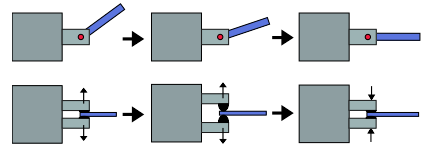
\includegraphics[scale=0.5]{appendices/pic/1-1}
  \caption*{
    \mtb{图1}通过控制两个手指的抓握所产生的夹持力来转动物体。
    上面一行展示机器人如何打开和关闭夹持器来控制由重力引起的物体旋转运动。
    该被控物体绕一个固定的旋转轴旋转,该旋转轴连接两个手指,如第二行所示。}
  \vspace{-0.3cm}
\end{figure}


在这篇论文中,我们提出了一种特殊的再抓取动作,称为旋转,
其目标是将被抓取的物体相对于机器人手旋转到一个指定角度的位置。
我们利用如图 1 所示的外部灵巧性来实现旋转,
利用被抓取物体质心产生的重力矩来旋转物体,
同时利用单自由度平行指夹具的夹持力作为制动机构来控制物体的转动轨迹。

旋转和其他在手操作的主要难题之一是如何处理未知的摩擦参数。
这是一种常见的情况,因为机器人可能需要抓取新对象或工具。
此外,由于摩擦参数与接触几何形状和压力分布等因素有关,
因此在实际测量时可能会有困难。

这激发了我们工作的主要动力。我们使用一个闭环自适应控制器进行旋转,
该控制器处理扭转摩擦参数估计不准确的问题。该控制方案需要用到视觉跟踪和
指尖触觉传感器。相较与我们之前使用闭环控制的方法$^{[5]}$,我们这次不再依耐一
些假设,如输入量的饱和。而且我们作出了以下改进,实现了增强的跟踪控制性能:

\begin{itemize}
  \item 利用软指力学改进了扭转摩擦模型。
  \item 结合触觉传感器来控制夹持力。
  \item 扭 转 摩 擦 系 数 的 实 时 修 正 。
				这 使 我 们 能 够 在 给 定 的 初 始 估 计 值 有误差的情况下,
				成功地旋转物体。
\end{itemize}


本文主要内容如下:第二节介绍该问题的相关研究工作,
第三节介绍系统的接触和动力学模型,第四节给出自适应控制律,第五节给出实验结果。
最后,我们在第六部分提出了我们的结论和未来的工作计划。


  % \appchapter{研究现状}
在手操作中,即重新定位机器人手中的物体,
一直是机器人学中的一个长期研究课题,涉及到建模、运动规划和控制等多个方面。
Tournassoud 等人的早期研究展示了可以通过在一个表面上通过反复地抓取
和放置来实现再抓取 $^{[6]}$。然而,这个过程可能会很耗时,
并且可行的再抓取姿态由物体能稳定地放置在该表面上的姿态决定。
因此,研究人员很快意识到需要更高级的灵巧操作技巧。
一种提出的解决方案是控制手指的运动,
通过滚动、滑动和在手指间移动来实现被抓取物体的重新定位$^{[7, 8]}$。

另一方面,其他研究提出了利用环境协助在手操作的想法。Brock 等人是最早
提出在外力作用下通过物体的受控滑动来增强机器人灵巧性的人之一$^{[9]}$。 Dafle 等
人定义了外部灵巧性这一概念,并展示了一个低自由度机器人手仍然可以利用重
力和环境约束等外部资源完成一组不同的原始动作,进而实现复杂的在手操作$^{[1]}$。
这种利用机器人环境的想法也被用于抓取情景中$^{[10]}$。

这些研究强调了接触和摩擦建模作为灵巧操作的核心内容的重要性。 
Goyal 提出了极限曲面的概念,极限曲面描述了可以让被抓取物体发生滑动的力旋的边界,
以及滑动发生时物体的运动方向的边界 $^{[11]}$。Howe 等人进一步发展了这些思想,
并提出了在操纵规划和控制时估计极限面的便于计算的方法$^{[12]}$。

在机械系统的摩擦识别和补偿方案设计中,也对摩擦建模进行了研究$^{[13, 14]}$。
然而,在这些研究中发展的控制技术不能直接应用到我们的工作中 ,
因 为 他 们 将 摩 擦 视 为 附加扰动,而在我们的研究中,摩擦代表一个控制输入。
从这个角度看我们的控制器与汽车上的防抱死制动系统(ABS)有一定的相似之处,
然而这些工作的目的是最大限度地提高轮胎和路面之间的牵引力$^{[15]}$。

触觉感知在机器人操作中也发挥了重要作用,部分原因是它在人类执行的最
基本的拾取和放置操作任务中发挥了重要作用$^{[16]}$。
许多研究都是通过触觉感知来解决滑动检测问题,
然而,这些研究的主要目的是在抓握控制中防止滑动,而不是控制滑动$^{[17, 18]}$。
一些工作也提出了摩擦参数的在线估计方法$^{[18]}$,但重点放在滑动摩擦力上,
而不是像我们的例子中的摩擦力矩。

近期有学者对具有外部灵巧性的在手操作进行了建模、机械设计和运动规划
等方面的研究。Dafle 等人研究了抓握推送的力学,分析了推送器与被控物体接触
的几何形状对物体滑动的影响 $^{[2]}$。Dafle 等人还设计了特别的指尖,使机器人能
够轻松地转换抓取方式,实现稳定地抓取物体或者让物体自由转动$^{[19]}$。

Shi 等人提出了一种运动规划框架,
该框架可以确定让物体相对于机器人手滑动一定距离时机器人手所需的加速度 $^{[4]}$。
这项工作解决了一个类似于我们的场景,即一个物体被两个手指捏住,
还能在三个平动自由度上调整物体相对于机器人手的位置。
虽然这项研究中的仿真实验验证了其提出的方法,但实验并没有达到预期的效果,
部分原因是缺乏反馈控制和触觉感知。

与我们的工作密切相关的还有 Holladay 等人提出的开环旋转框架$^{[3]}$。在他的
研究中,机器人首先在夹持在一个物体的表面,然后按照预先计算的运动轨迹将其
举起。如果使用开环控制,没有对物体姿态的在线跟踪,也没有对夹持力的控制,
那么物体只能在一组离散的稳定姿态之间旋转。

与近年来采用开环运动规划策略的文献$^{[3,4]}$相比,我们着重于采用具有在
线视觉跟踪和触觉传感的自适应反馈控制来控制抓取力。


  \includepdf[pages={1,2}]{appendices/article.pdf}


  % ===== Back | 书后部分 =====
  % \backmatter
\end{document}

!!!!! ------ Common commands: --------!!!!!
\syntaxonly		% 只检查语法
\includeonly{sections/section-01,appendixes/appendix-01}	% Only coding these sections

!!!!! ------- Note: ------- !!!!!

